\section{Motivation}

\begin{frame}
	\frametitle{Motivation}
	
	\begin{center}
		\begin{tikzpicture}
			\node at (0,0) [draw=white,ultra thick,inner sep=0pt] {
\includegraphics[scale=0.37]{images/Motivation1}};
		\end{tikzpicture}
	\end{center}
\end{frame}

\begin{frame}
	\frametitle{Motivation}
	
	\begin{center}
		\begin{tikzpicture}
			\node at (0,0) [draw=white,ultra thick,inner sep=0pt] {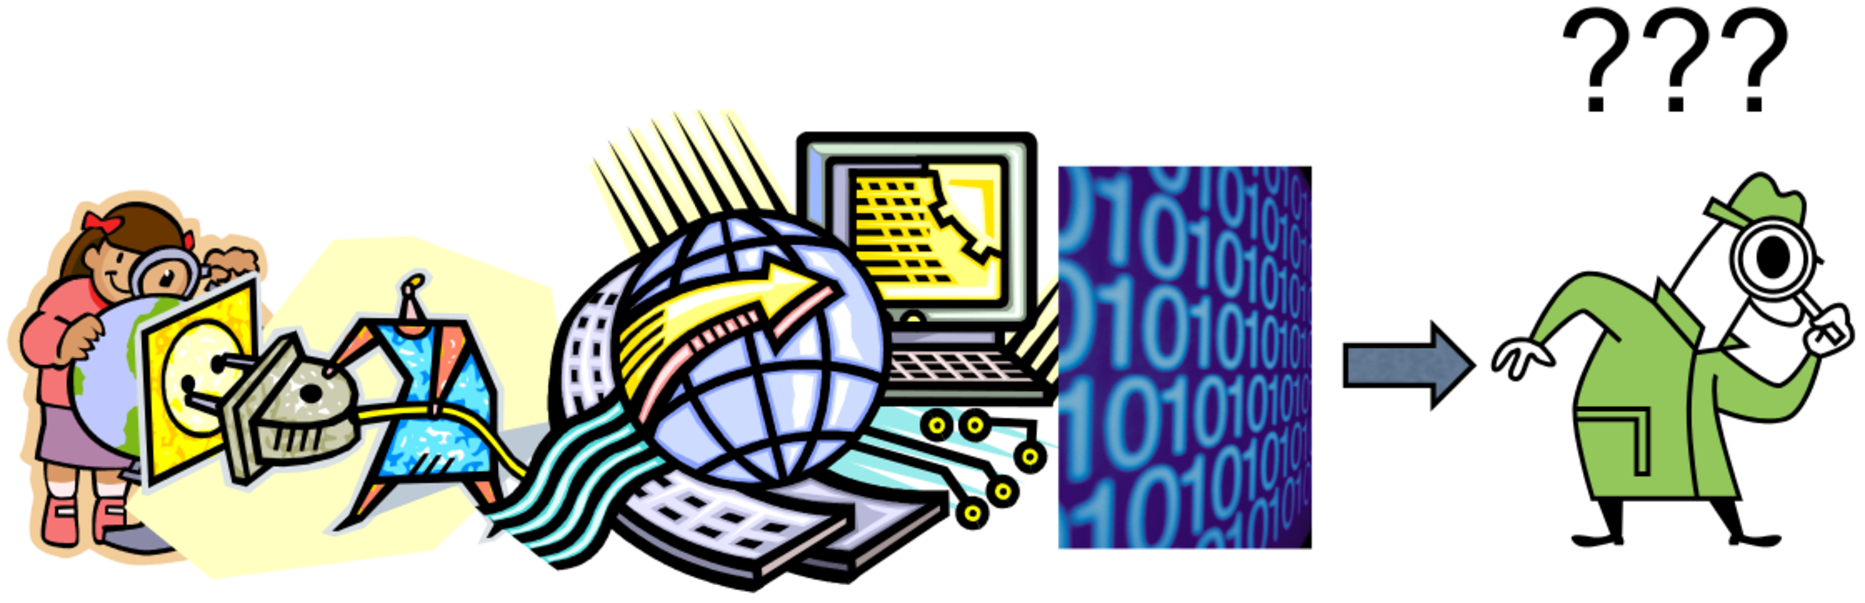
\includegraphics[scale=0.37]{images/Motivation2}};
		\end{tikzpicture}
	\end{center}
\end{frame}

\begin{frame}
	\frametitle{Motivation}
	
	\vspace{-0.03cm}
	
	\begin{center}
		\begin{tikzpicture}
			\node at (0,0) [draw=white,ultra thick,inner sep=0pt] {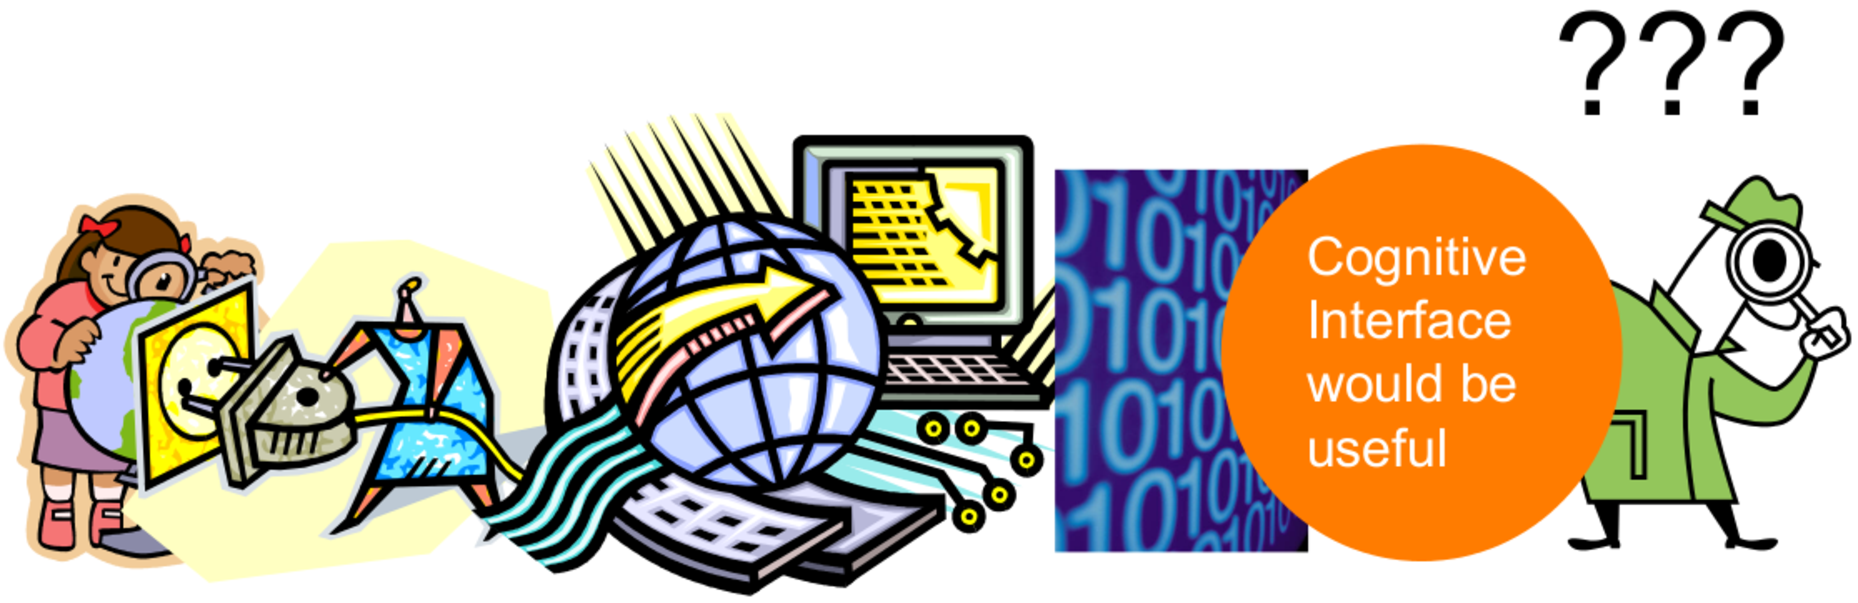
\includegraphics[scale=0.37]{images/Motivation3}};
		\end{tikzpicture}
	\end{center}
\end{frame}

\begin{frame}
	\frametitle{Motivation}
	
	\begin{center}
		\begin{tikzpicture}
			\node at (0,0) [draw=white,ultra thick,inner sep=0pt] {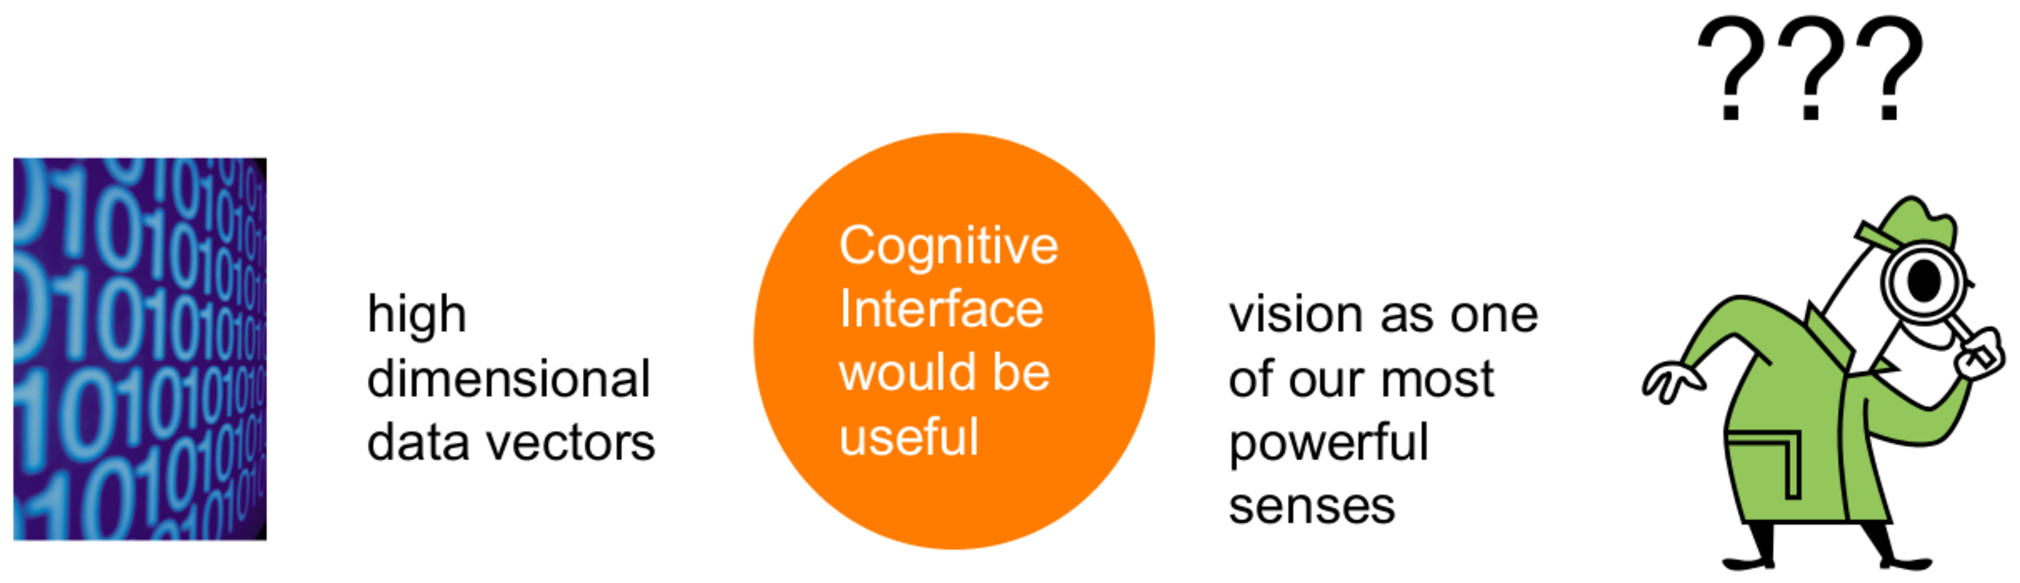
\includegraphics[scale=0.34]{images/Motivation4}};
		\end{tikzpicture}
	\end{center}
\end{frame}

\begin{frame}
	\frametitle{Example}
	
	\begin{center}
		\begin{tikzpicture}
			\node at (0,0) [draw=white,ultra thick,inner sep=0pt] {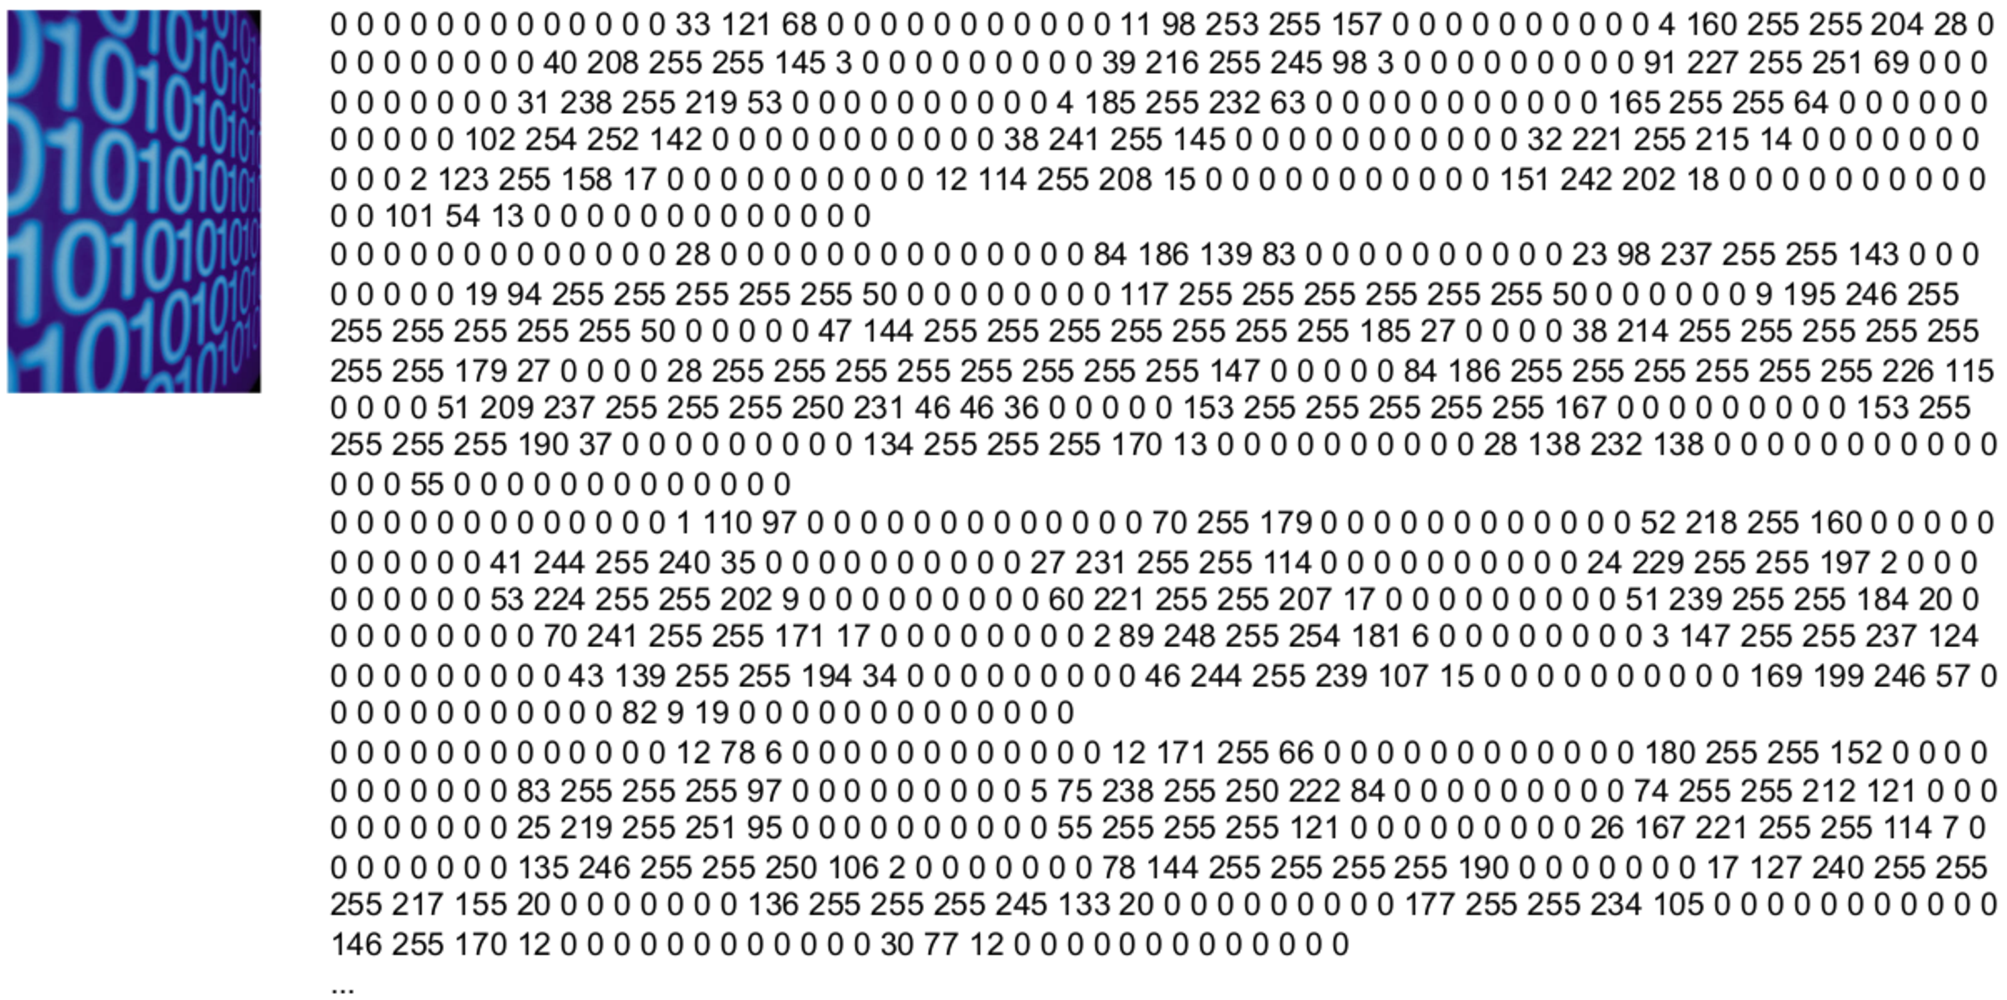
\includegraphics[scale=0.34]{images/Example1}};
		\end{tikzpicture}
	\end{center}
\end{frame}

\begin{frame}
	\frametitle{Example}
	
	\vspace{0.8cm}
	
	Each vector represents a 16x16 grey-valued image.
	
	\begin{center}
		\begin{tikzpicture}
			\node at (0,0) [draw=white,ultra thick,inner sep=0pt] {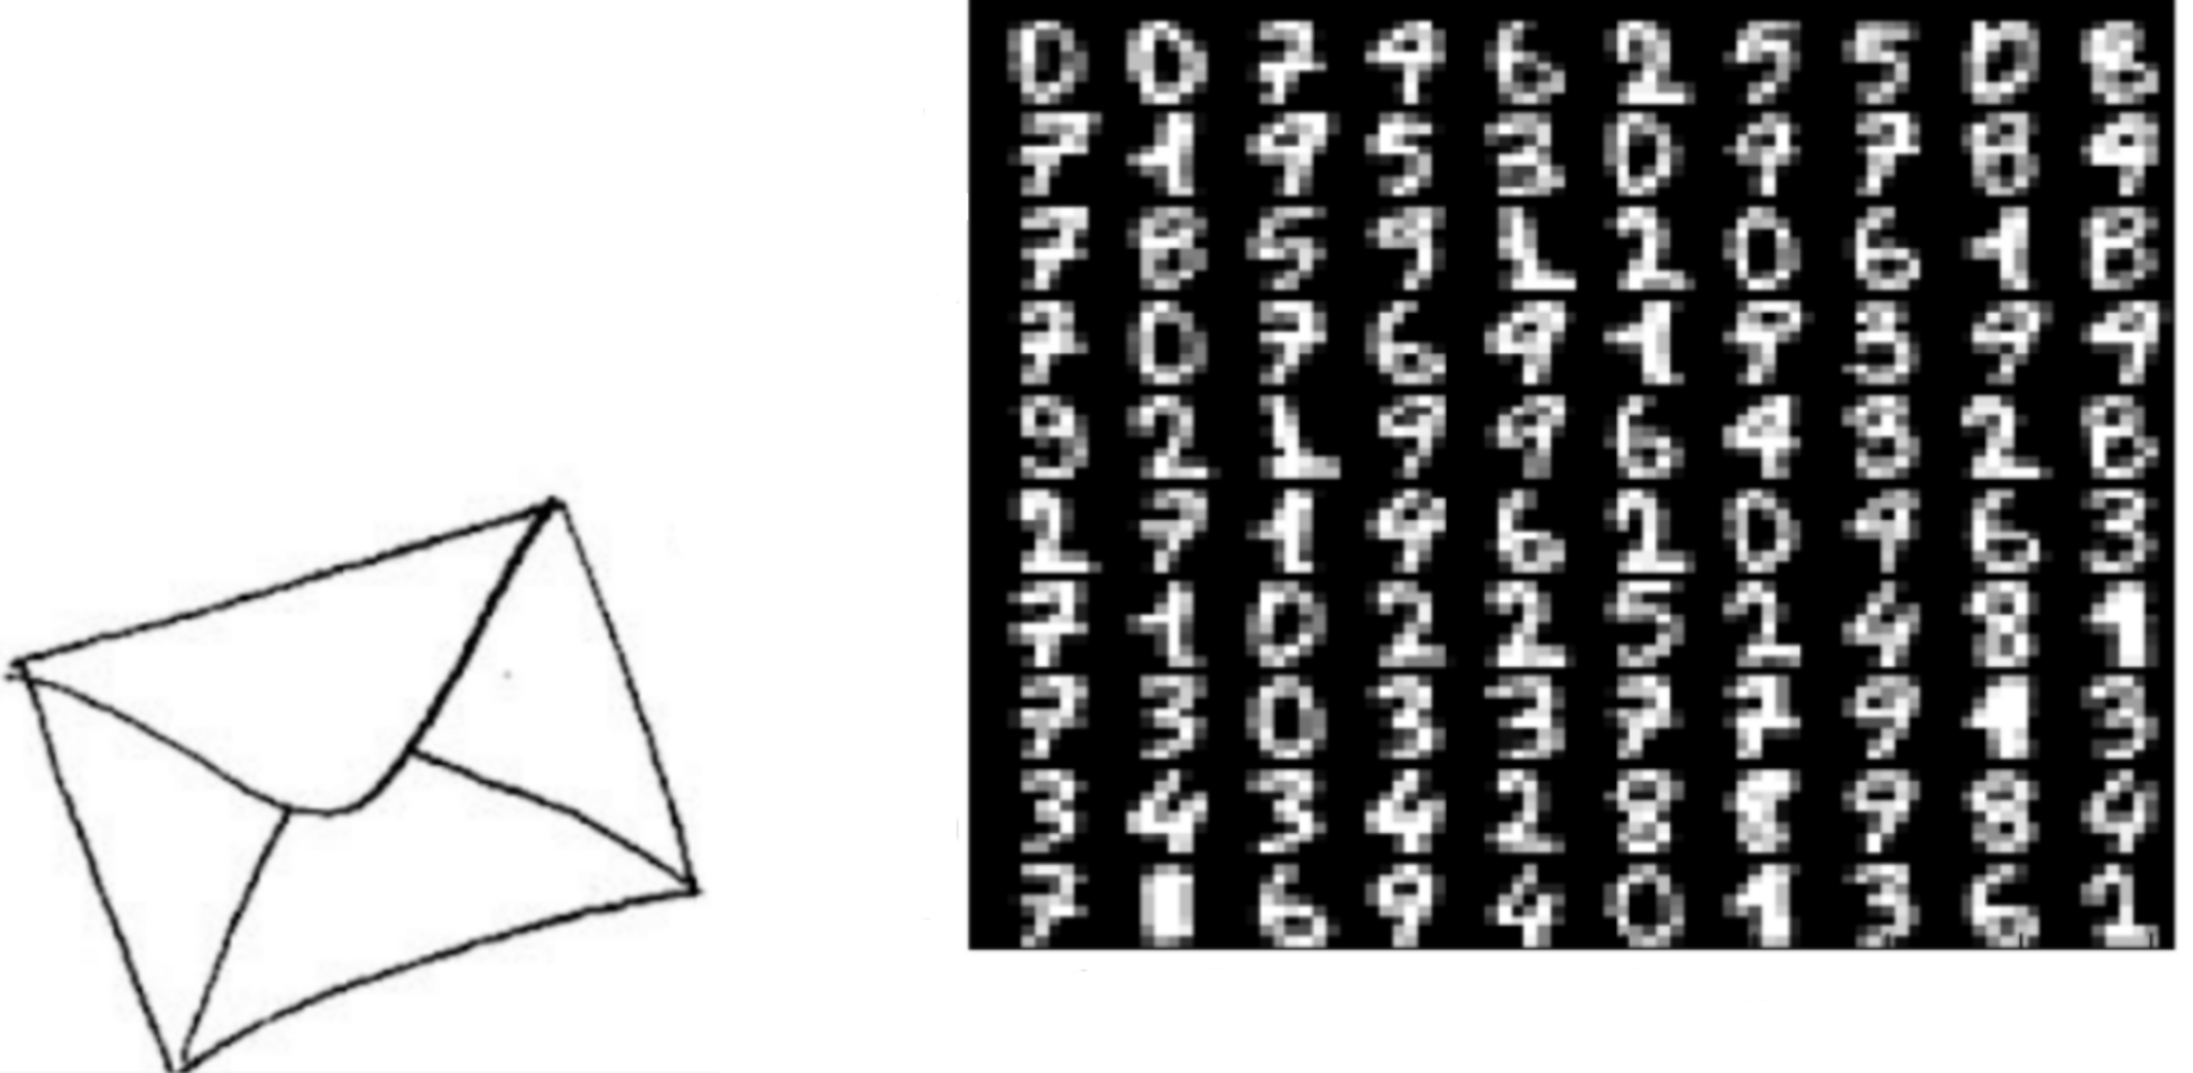
\includegraphics[scale=0.28]{images/Example2}};
		\end{tikzpicture}
	\end{center}
\end{frame}

\begin{frame}
	\frametitle{Another example}
	
	\vspace{0.4cm}
	
	How many different clusters?
	
	\vspace{0.4cm}
	
	\begin{center}
		\begin{tikzpicture}
			\node at (0,0) [draw=white,ultra thick,inner sep=0pt] {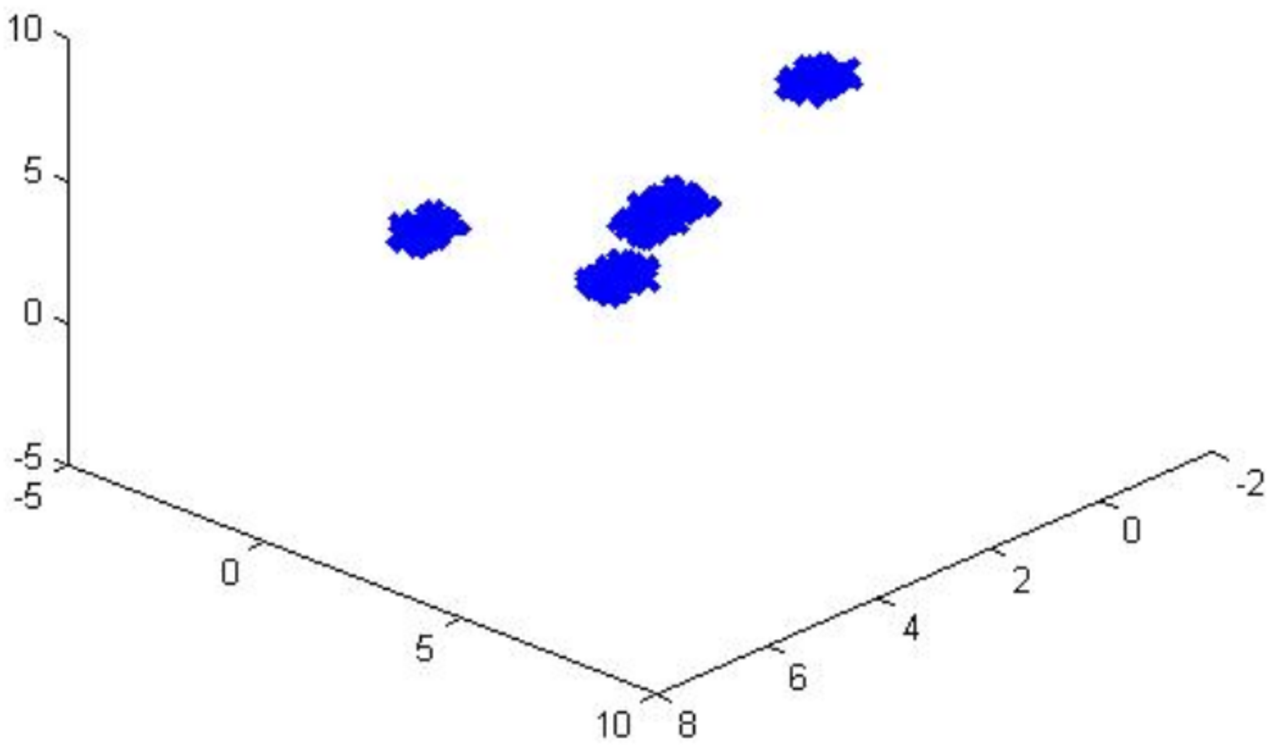
\includegraphics[scale=0.34]{images/Example3}};
		\end{tikzpicture}
	\end{center}
\end{frame}

\begin{frame}
	\frametitle{Another example}
	
	\textbf{Wrong answer!} The chosen visualization is important.
	
	\vspace{0.4cm}
	
	\begin{center}
		\begin{tikzpicture}
			\node at (0,0) [draw=white,ultra thick,inner sep=0pt] {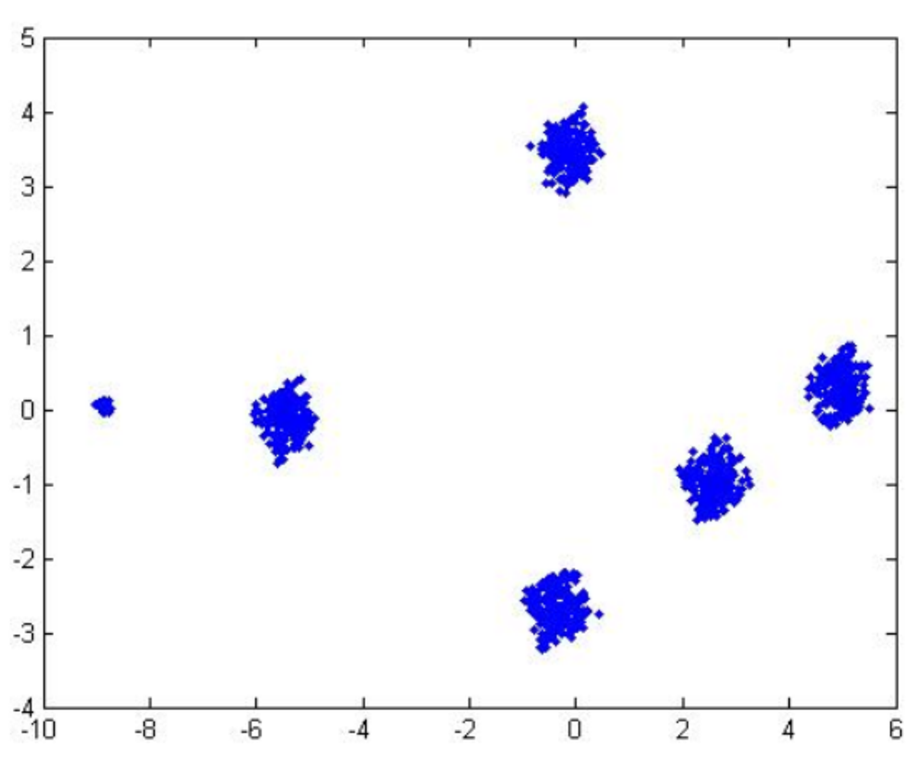
\includegraphics[scale=0.28]{images/Example4}};
		\end{tikzpicture}
	\end{center}
\end{frame}

\begin{frame}
	\frametitle{Dimensionality reduction}
	
	\vspace{0.2cm}
	
	\begin{block}{Objective}
		Mapping high-D data to 2-D (or 3-D) data such that \textbf{as much information as} possible is preserved
	\end{block}
	
	\begin{center}
		\begin{tikzpicture}
			\node at (0,0) [draw=white,ultra thick,inner sep=0pt] {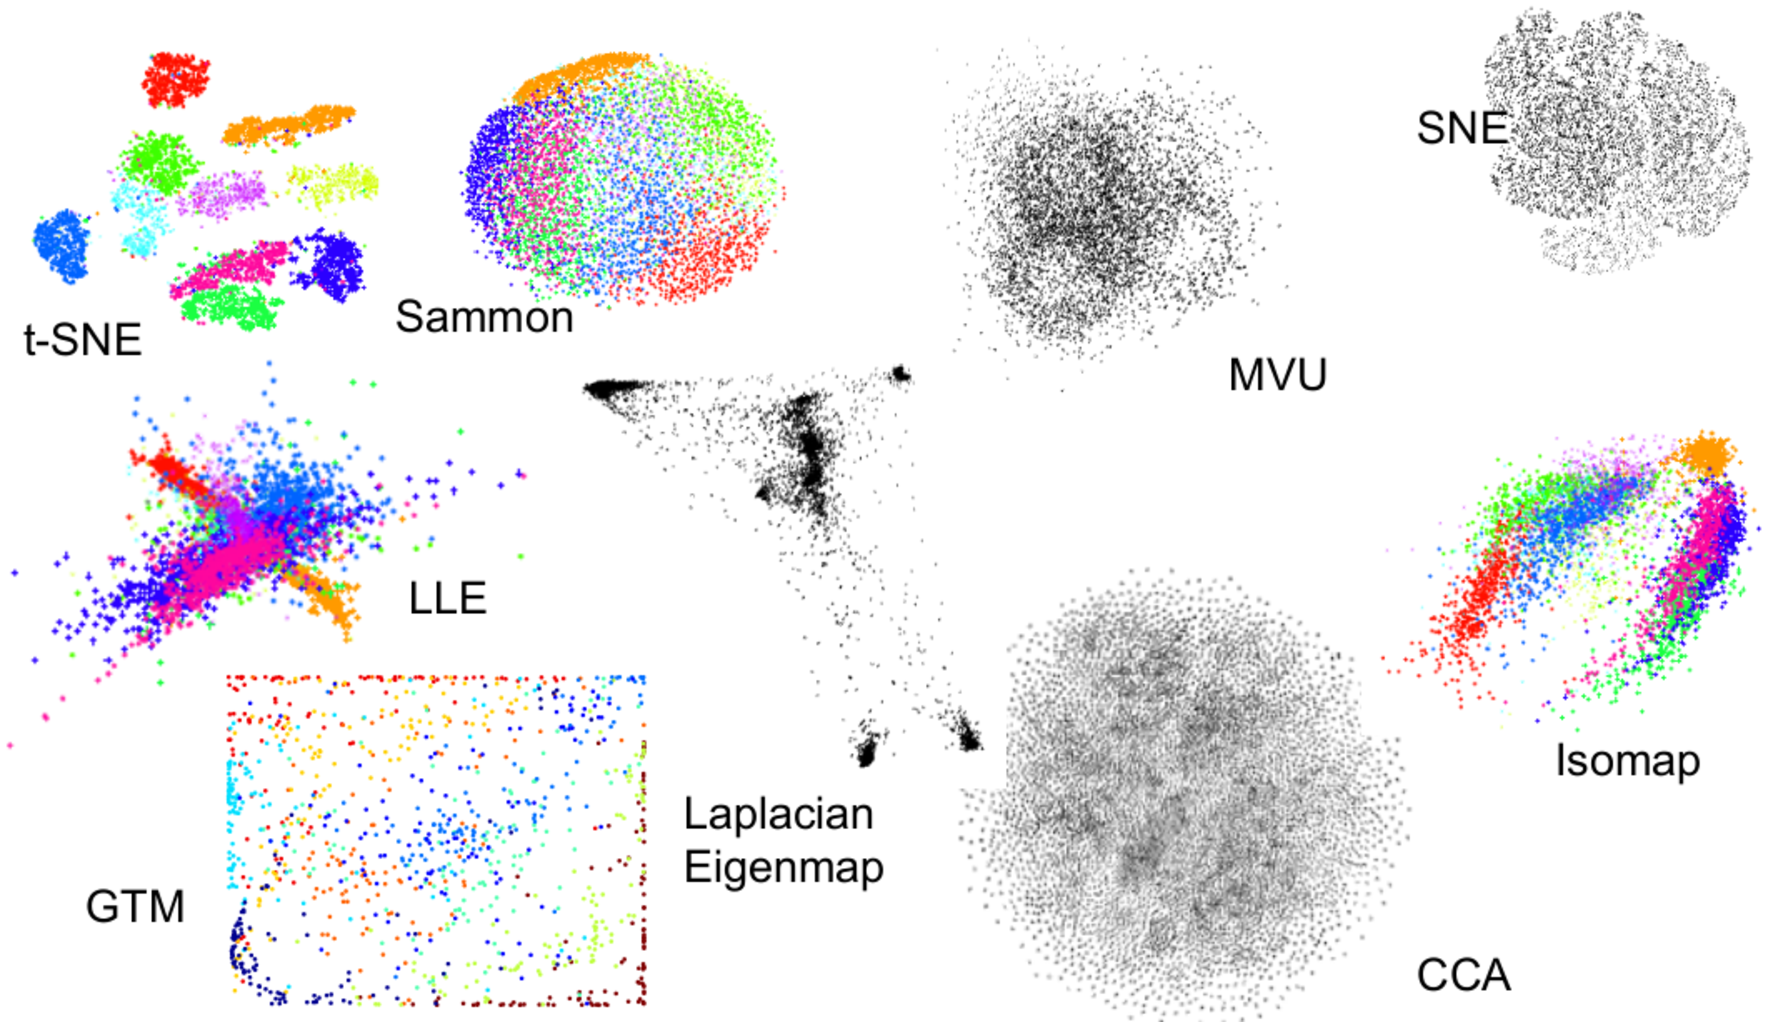
\includegraphics[scale=0.3]{images/Methods}};
		\end{tikzpicture}
	\end{center}
\end{frame}

\begin{frame}
	\frametitle{Several methods for a dimensionality reduction}
	
	\vspace{0.4cm}
	
	\begin{center}
		\begin{tikzpicture}
			\node at (0,0) [draw=white,ultra thick,inner sep=0pt] {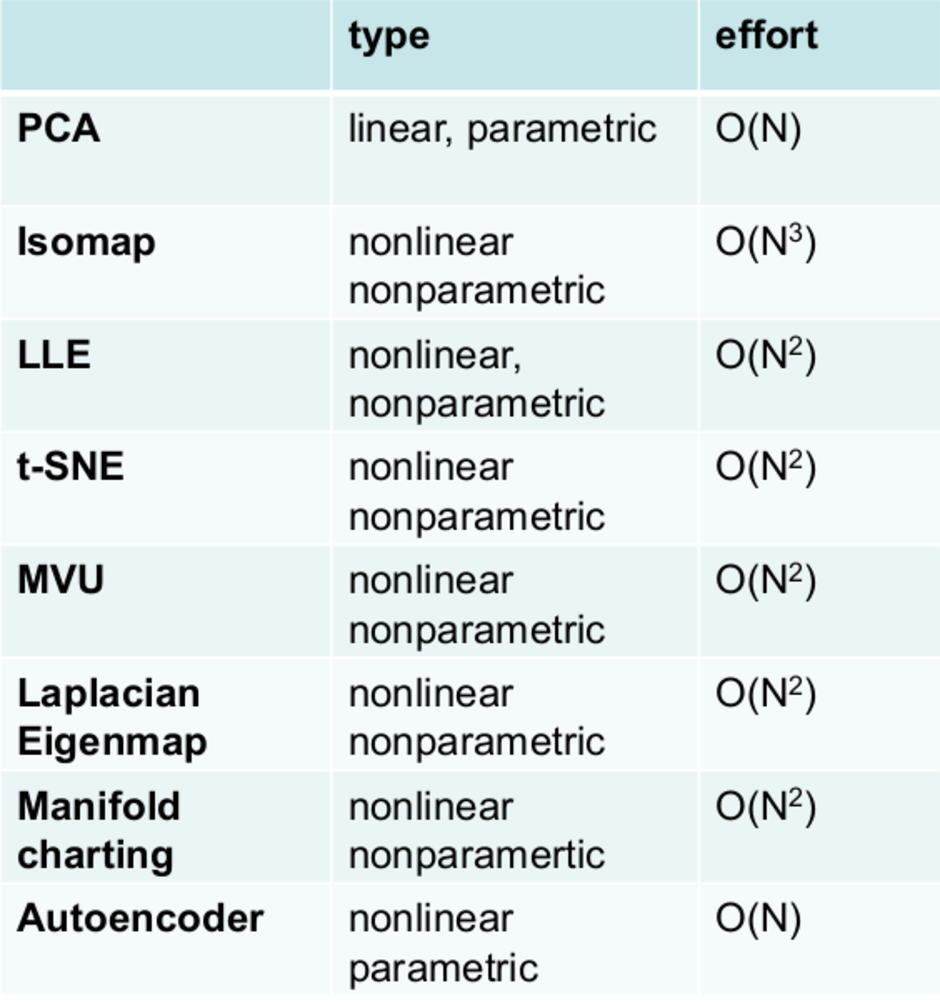
\includegraphics[scale=0.4]{images/TableMethods}};
		\end{tikzpicture}
	\end{center}
\end{frame}
